\documentclass{article}
\usepackage{listings}
\usepackage[utf8]{inputenc}
\usepackage{ amssymb }
\usepackage{amsfonts}
\usepackage{graphicx}

\title{Sistemas Distribuidos y Verificación \\ Tarea 1}
\author{Fabián Romero Jiménez}
\begin{document}
\maketitle

\begin{enumerate}

\item[\bf{Problema 1}] En clase se vio el complejo de la Figura 1, donde los mundos eran compatibles si difieren en un bit.\\

\begin{center}
  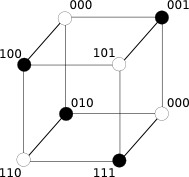
\includegraphics{cubo1.png}\\
  Figura 1
\end{center}

%\begin{figure}[p]
%    \centering
%    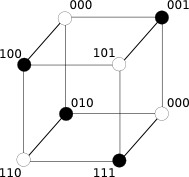
\includegraphics{cubo1.png}
%    \caption{Figura 1}
%    \label{fig:cubo1}
%\end{figure}

\begin{enumerate}

\item Como sería el complejo si los mundos son compatibles cuando las vistas(etiquetas) difieren en 2 bits.\\

Demostraremos que como el proceso negro solo puede mentir en el bit del medio, el proceso blanco nunca podrá ser engañado, es decir, en cada caso puede saber si el proceso negro esta mintiendo o no y por lo tanto saber exactamente el estado del proceso negro, por lo que el modelo de conocimiento será exactamente el complejo visto en clase (Figura 2).\\

\begin{center}
  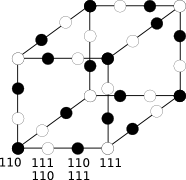
\includegraphics{cubo2.png}\\
  Figura 2
\end{center}

\emph{Demostración:} Si el mensaje difiere en 0 bits, dado que el proceso blanco sabe que sus visiones difieren en exactamente un bit, puede deducir que el proceso negro esta mintiendo (y sabe que esto es en el bit del medio). Si el mensaje difiere en 1 bit, el proceso blanco sabe que el proceso negro no esta mintiendo.  Si difiere en 2 bits tambien sabe que esta mintiendo y no puede diferir en 3 bits, por que es sabido que inicialmente difieren en exactamente un bit y se puede mentir en solo uno, por lo que a lo más podrá diferir en 2 bits.\\

Si queremos representar no el conocimiento, sino la comunicación, donde son distinguibles el mundo donde el proceso negro dijo la verdad y donde dijo una mentira (La distinción será que hay dos mundos, en ambos el proceso blanco sabe exactamente la etiqueta del proceso negro, pero en un mundo sabe que el proceso negro mintio y en el otro sabe que el proceso negro dijo la verdad). El complejo sería el de la Figura 3.

\begin{center}
  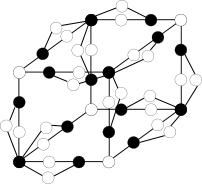
\includegraphics{cubo3_1_1.png}\\
  Figura 3
\end{center}

Que es mas fácil visualisar en la Figura 4

\begin{center}
  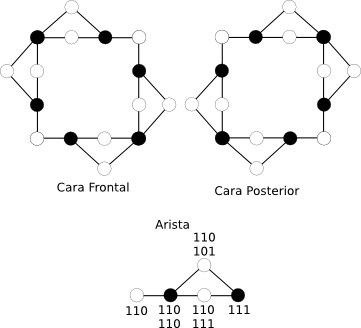
\includegraphics{cubo3_2.png}\\
  Figura 4
\end{center}

Donde cada arista, aquí solo representada la que une los datos 110 con 111, pero en general es equivalente a cada una de ellas representa las comunicaciones, que son las que ya se habian descrito en el caso visto en clase mas una ``oreja'' que representa 2 mundos más, en aquel que el proceso negro miente y en aquel que miente, pero ese mensaje se pierde.

\item{Como sería el complejo si los mundos son compatibles cuando las vistas(etiquetas) difieren en 2 bits.}\\
En este caso, por paridad, se crean 2 complejos disjuntos y complementarios, uno que tiene etiquetas con una cantidad par de 1's y otro con una cantidad impar de 1's, Esto es asi puesto que si cambian 2 bits hay dos casos, que estos sean diferentes y al cambiarlos la cantidad de 1's se conserva o que los bits sean iguales en este caso la cantidad de 1's aumenta en dos o bien disminuye en dos pero preserva la paridad, por lo que si cambian 2 bits la etiqueta vecina conserva la paridad de 1's.
Como se muestra en la Figura 5:


\begin{center}
  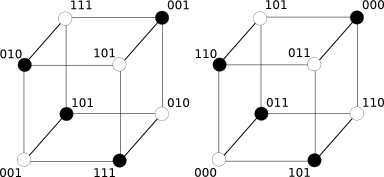
\includegraphics{cubo4.png}\\
  Figura 5
\end{center}

\end{enumerate}

\item[\bf{Problema 2}] Considera el complejo de la Figura 6, que representa la entrada de una tarea tal que a la salida sólo un proceso regresa cero y los otros dos regresan 1.

\begin{center}
  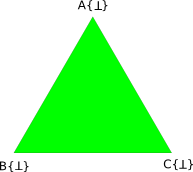
\includegraphics{figura6.png}\\
  Figura 6
\end{center}


\begin{enumerate}
\item Da un algoritmo que resuelva la tarea, y demuestra que es correcto.

El modelo de comunicación es síncrona y de memoria compartida.
El algoritmo es el siguiente:
En cada turno, cada proceso escribe un número aleatorio y su nombre en la memoria compartida, repitiendo hasta que sean todos distintos, cuando lo son.\\

Aqui por simplicidad, se supone la existencia de una función ``rand'' genuinamente aleatoria, en la practica podria tomar una función semialeatoria con una semilla inteligentemente elejida o alguna forma de determinar unicamente la identidad del proceso como semilla, o el mismo identificador del proceso como resultado de ``rand'' si sabemos que tal identificador es único.
\newpage
Programa:\\
\begin{lstlisting}[frame=single]
do {
  // toma un valor aleatorio
  value=rand();                        
  // lo escribe en la memoria compartida
  write(this.name, value);             
  // espera a que termine el turno
  wait(1);                   
  // verifica que        
} while(all_unique(read_values())==false); 
  // determina si es el menor
  is_min=value==min(read_values());
  // si lo es pone en su salida un 0, o bien
  // 1 en caso contrario
  out=(is_min)?0:1;       
\end{lstlisting}

{\bf Demostración de correctitud:}
Para salir del ciclo while se requiere que todos los números sean distintos por lo que todos los procesos salen en el mismo turno del ciclo while.\\
Dado que la función ``rand()'' es genuinamente aleatoria, no podría quedarse dentro del ciclo ``while'' infinitamente.\\
Una vez que sale del ciclo, dado que los 3 números son distintos hay exactamente uno que es el menor y solo el pone un 0 a la salida, los otros 2 ponen un 1, por lo que la salida siempre tendrá un 0 y dos un 1 $\blacksquare$.

\item Dibuja el complejo de salida.\\
Denotamos $A1$ el proceso con nombre $A$ y salida $1$ y equivalentemente a los demas, así, los vértices con un uno, A1, B1, C1, viven cada cual en 2 mundos, por ejemplo A1 vive en ${(A,1),(B,0),(C,1)}$ y en ${(A,1),(B,1),(C,0)}$  

\begin{center}
  
  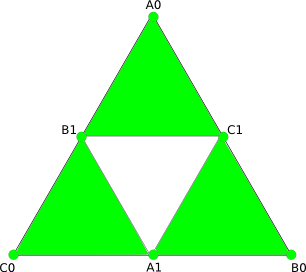
\includegraphics{figura7.png}\\
  Figura 7
\end{center}

\end{enumerate}

\item[\bf{Problema 3}] Recuerden el problema de las esposas infieles (a.k.a. Niños enlodados, Muddy Children). Sea n el número de caballeros y k el número de caballeros engañados. Demuestra por inducción, que si el cantinero da como información inicial que hay al menos 3 caballeros engañados, entonces en la ronda k-3 se levantan los k engañados. Escribe el pseudo código del algoritmo que ejecutan

\item[\bf{Demostración}] 
Observemos que en todo momento, cada uno de los caballeros sabe que al menos hay tantos engañados como engañados ve, y que a lo más, hay los que ve mas uno (el mismo).
Por lo que siempre sabe con certeza una cota máxima que es el número de engañados que ve más uno.

Demostraremos por inducción sobre el número de rondas que han pasado que:\\
Si hay k caballeros engañados, en cada ronda s $(0 \le s \le k)$ sabe que hay al menos (s+3) engañados y en la ronda k-3 sabe que si se llego hasta ahi, el es uno de los engañados y puede levantarse (simultaneamente que todos los demás).\\

Caso base: s=0 rondas.\\
Cada uno de los caballeros engañados, ve a otros (k-1) engañados y sabe que hay al menos 3 engañados, asi que si k=3 sabe inmediatamente (en tiempo 0) que el es engañado y se levanta, si k>3, sabe que el ve a k y que el mismo puede ser engañado, pero que como por el momento la cota es 3, todavia no puede levantarse\\

Hipotesis de inducción: Supongamos que es correcto hasta el caso de n rondas y demostremos con n+1.\\
Cada uno de los caballeros engañados, ve a otros (k-1) engañados y sabe que hay al menos n+3 engañados, asi que si k=n+3 sabe inmediatamente que el también es engañado y se levanta, si k>n+3, sabe que el ve a k y que el mismo puede ser engañado, pero que como por el momento por hipotesis de inducción la cota es n+3 , todavia no puede levantarse y espera una ronda más $\blacksquare$.\\




\item[\bf{Problema 4}] Supongamos que tenemos una gráfica con vértices etiquetados que es un camino (vértices con grado a lo más 2). Las etiquetas válidas son 0,1.\\
También supongamos que los extremos de la gráfica esta uno etiquetado con 0 y otro con 1. Demuestra que hay un número impar de aristas que sus vértices tienen etiquetas distintas. (Hint: hacer una suma de etiquetas).

\item[\bf{Respuesta}] 
Pongamos en cada arista $e_i$ la suma de sus vertices, de tal forma que será 0 si ambos vértices son 0, en 1 si son distintos y en 2 si ambos son 1, es decir, cada arista tendra un número par (0 ó 2) si ambos vértices son iguales y un número impar (1) si son distintos.

También tenemos que: $\sum_{i=0}^{i=k} e_i =v_o+2 \sum_{i=0}^{i=k} v_i + v_k $ puesto que cada vértice, excepto los extremos se cuentan 2 veces, uno en cada arista que esta.

pero por descripción del problema $v_0+v_k=1$, asi que $\sum_{i=0}^{i=k} e_i =1+2 \sum_{i=0}^{i=k} $ por lo que la suma de las aristas es un numero impar.\\

Pero solo las aristas cuyos vértices tengan etiquetas distintas tienen un numero impar (1), por lo que podemos deducir que hay un numero impar de dichas aristas ya que la unica forma de sumar un numero impar es con un numero impar de impares como sumandos $\blacksquare$



\item[\bf{Problema 5}] Ana, Bety y Carla toman cada uno una carta de un paquete de 3 cartas. Las 3 cartas 0,1,2.

\begin{itemize}
\item Describe el complejo de todas las posibles configuraciones iniciales
(es decir, todas las posibles formas en que Ana, Bety y Carla tienen
cada uno una carta). El complejo consiste de triángulos, cada uno
con 3 vertices etiquetados A,B y C.

El complejo como se muestra en la figura 8, podemos pegar la linea de arriba y abajo y los extremos izquierdos y derecho.

\begin{center}
  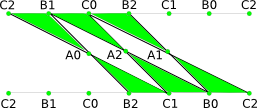
\includegraphics{figura8.png}\\
  Figura 8
\end{center}

Otra forma de verlo es como superponer los 3 hexagonos de la figura 9

\begin{center}
  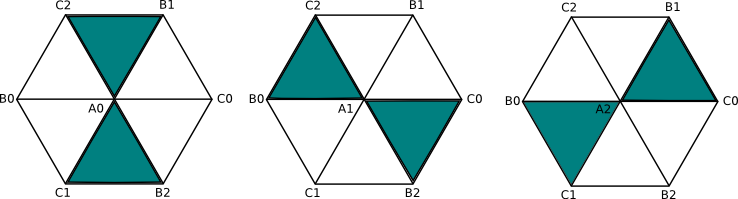
\includegraphics{figura9.png}\\
  Figura 9
\end{center}

aDonde los puntos B's y C's son los mismos, pero los puntos A0,A1 y A2 no son coplanares, son como 3 capas.

\item Supongamos que Ana dice publicamente ``No tengo la carta 1''. Anali-
za como cambia el complejo inicial después de este anuncio, y explica
que sabe cada uno después del anuncio (acerca de las cartas de los
demás).\\

Es el mismo complejo anterior eliminando el hexágono que tiene como centro A1, como se muestra en la figura 10.
\begin{center}
  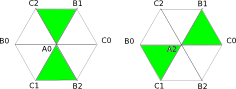
\includegraphics{figura10.png}\\
  Figura 10
\end{center}

\item Considera el anuncio, Bety dice ``Sigo sin saber la carta de Ana''.
Explica en que estados globales es posible que Bety haga este anuncio
sin mentir, y en esos estados, cual seria el efecto de hacer el anuncio
(como cambia el complejo y que sabe cada participante).\\
\end{itemize}

En el caso de que Bety no tenga la carta 1, entonces sabe que Carla debe de tenerla y existen los dos mundos de la figura 11, pero Bety sabe bien cual de ellos es el caso.

\begin{center}
  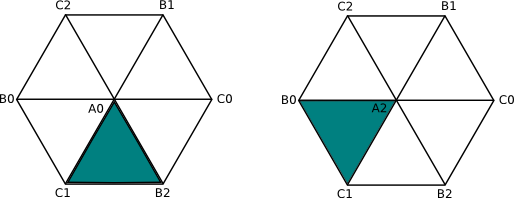
\includegraphics{figura11a.png}\\
  Figura 11
\end{center}

En el caso de que Bety si la tenga, pues los dos mundos posibles que se muestran en la 
figura 11 siguen subsistiendo.

\begin{center}
  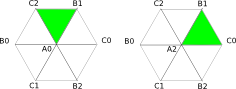
\includegraphics{figura11.png}\\
  Figura 11
\end{center}

\end{enumerate}
\end{document}
